\documentclass[journal]{IEEEtran}
\IEEEoverridecommandlockouts
\usepackage{cite}
\usepackage{amsmath,amssymb,amsfonts}
\usepackage{algorithmic}
\usepackage{graphicx}
\usepackage{textcomp}
\usepackage{xcolor}
\usepackage[justification=centering]{caption}
\def\BibTeX{{\rm B\kern-.05em{\sc i\kern-.025em b}\kern-.08em
    T\kern-.1667em\lower.7ex\hbox{E}\kern-.125emX}}
\begin{document}

\title{Dual-core machine learning accelerator for attention mechanism}

% Author order matches Word draft (team list); adjust as needed for final submission rules.
\author{
    \IEEEauthorblockN{Shreeya Ajay Bhonsle (A69040642)}
    , \IEEEauthorblockN{Chi-Han Chiu (A69036037)}
    , \IEEEauthorblockN{Nikhita Neelakanta (A69041742)}
    , \IEEEauthorblockN{Ming-Yang Wu (A16504833)}
    , \IEEEauthorblockN{Bing-Cheng Chiang (A69040193)}
    , \IEEEauthorblockN{Wen-Chieh Lo (A69042225)}
}

\maketitle

\section{Introduction}
This report summarizes RTL design, synthesis, place-and-route, and verification for a dual-core attention accelerator.
The following sections follow the course milestone flow (single core through sparsity-aware attention), merging the LaTeX report structure with the project outline document.
Placeholder figures use \texttt{temp.png} where a dedicated asset is not yet checked in.

% ═══════════════════════════════════════════════════════════════════════════
\section{Step 1: Single Core RTL, Synthesis \& PNR}
Post-PnR layout, GLS waveform, and terminal output for the single-core design are shown below, with summary metrics in Table~\ref{tab:s1}.

\begin{figure}[htbp]
    \centerline{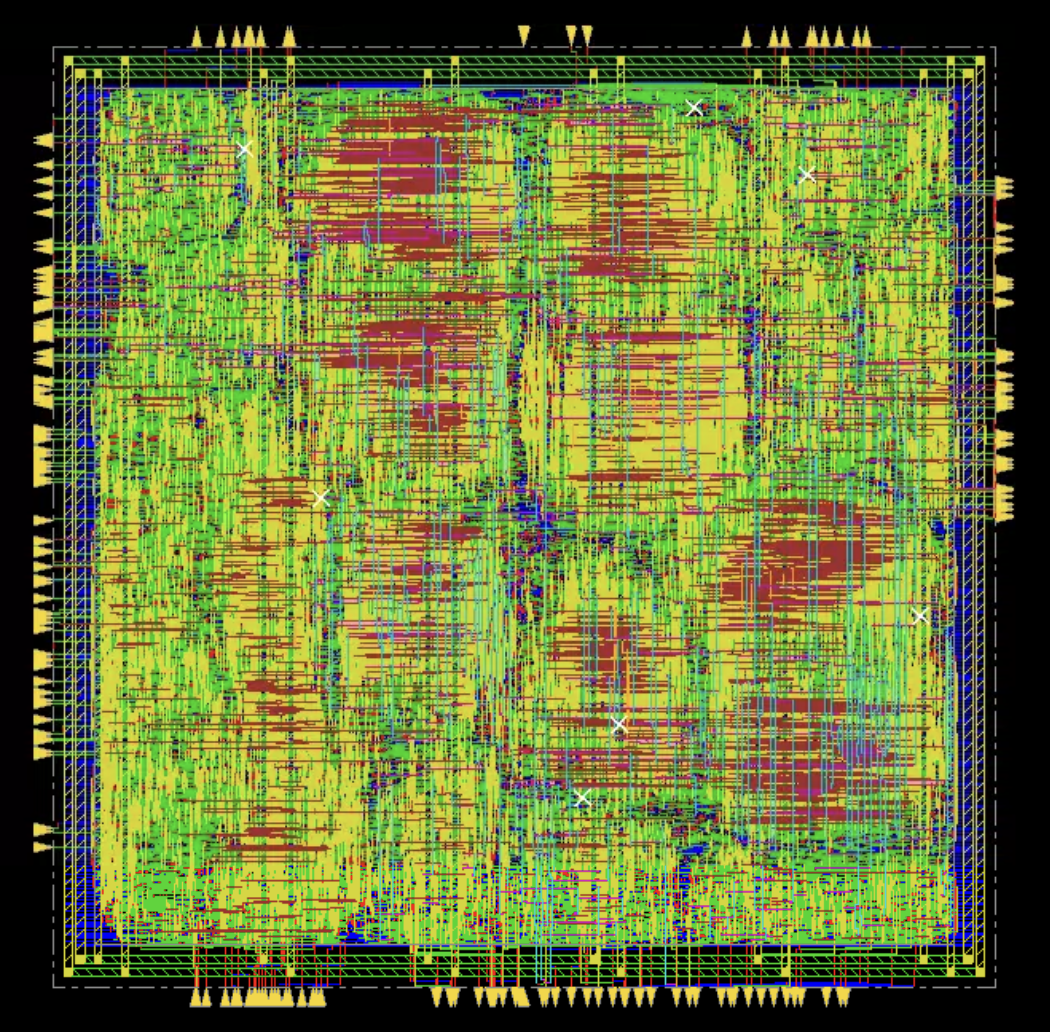
\includegraphics[width=0.30\textwidth]{Step1_images/Step1corelayout.png}}
    \caption{Single-Core Layout (post-PnR).}
    \label{fig:s1_layout}
\end{figure}

\begin{figure*}[htbp]
    \centerline{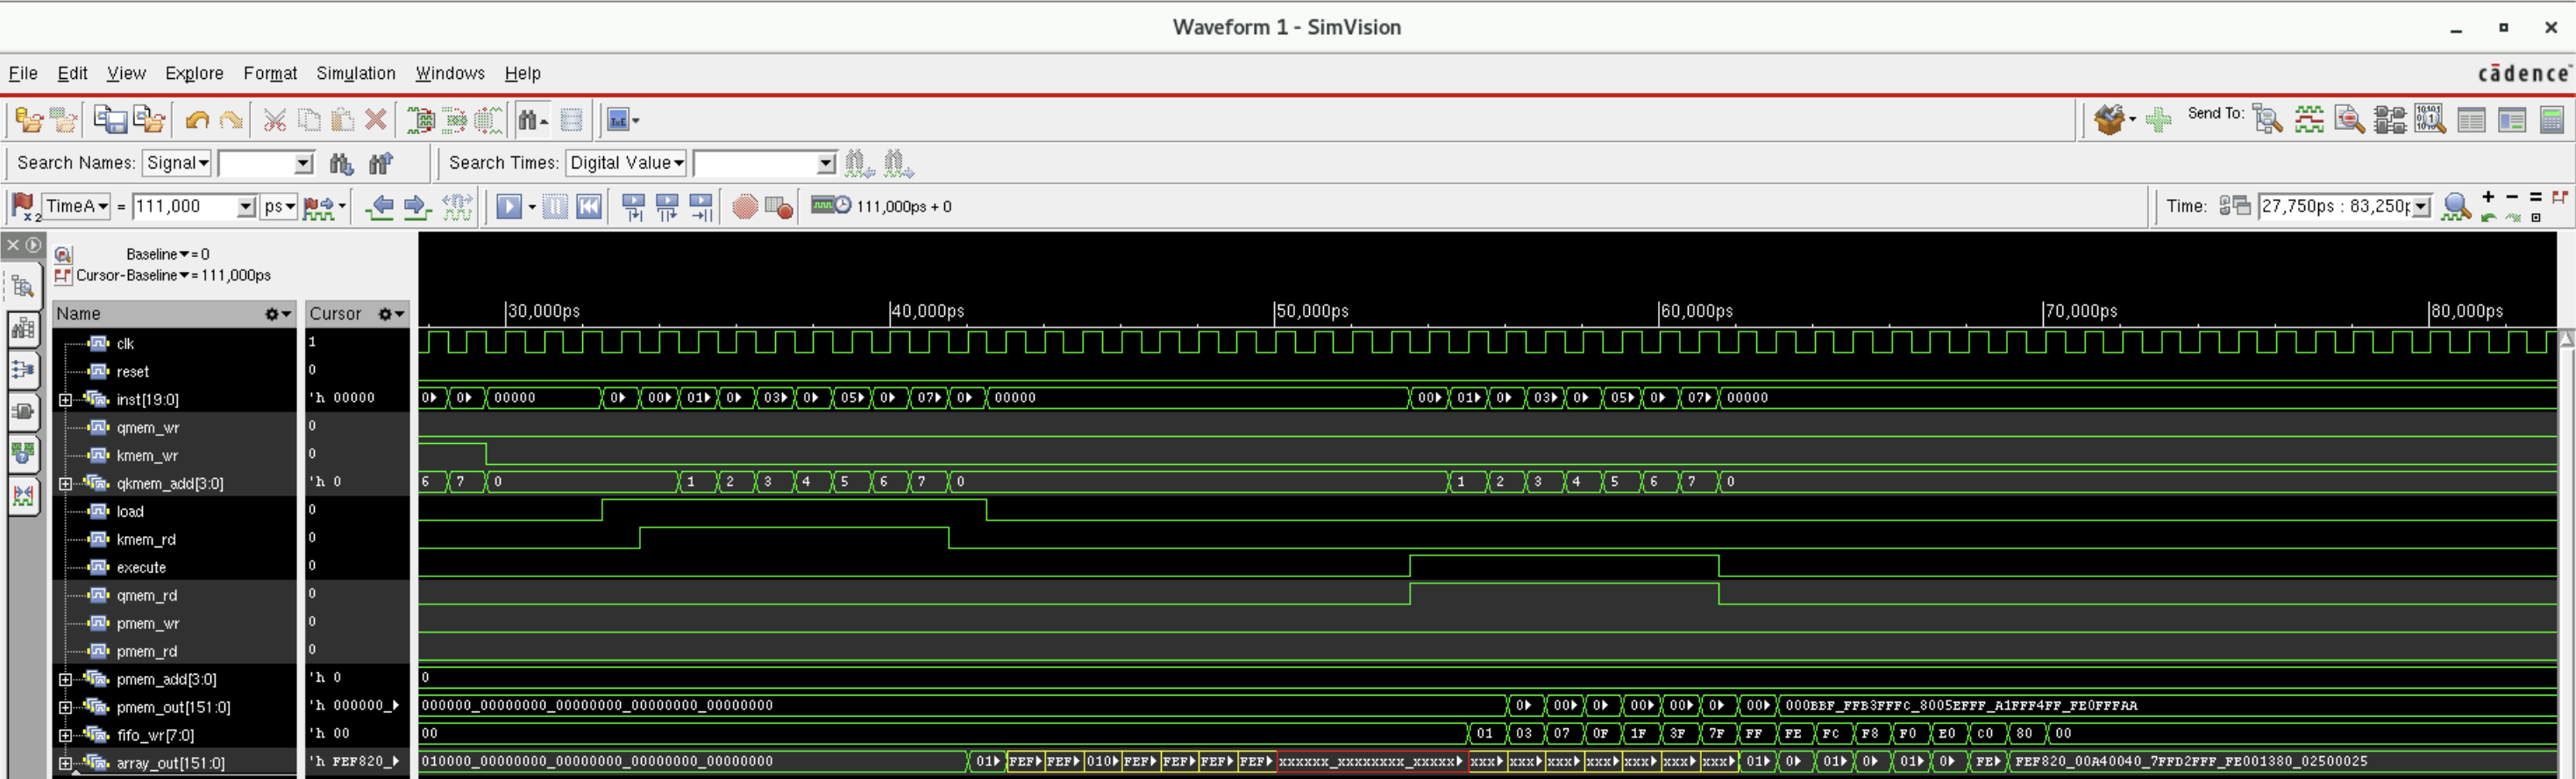
\includegraphics[width=1.0\textwidth]{Step1_images/Step1waveform.png}}
    \caption{Single-Core GLS Waveform.}
    \label{fig:s1_wave}
\end{figure*}

\begin{figure}[htbp]
    \centerline{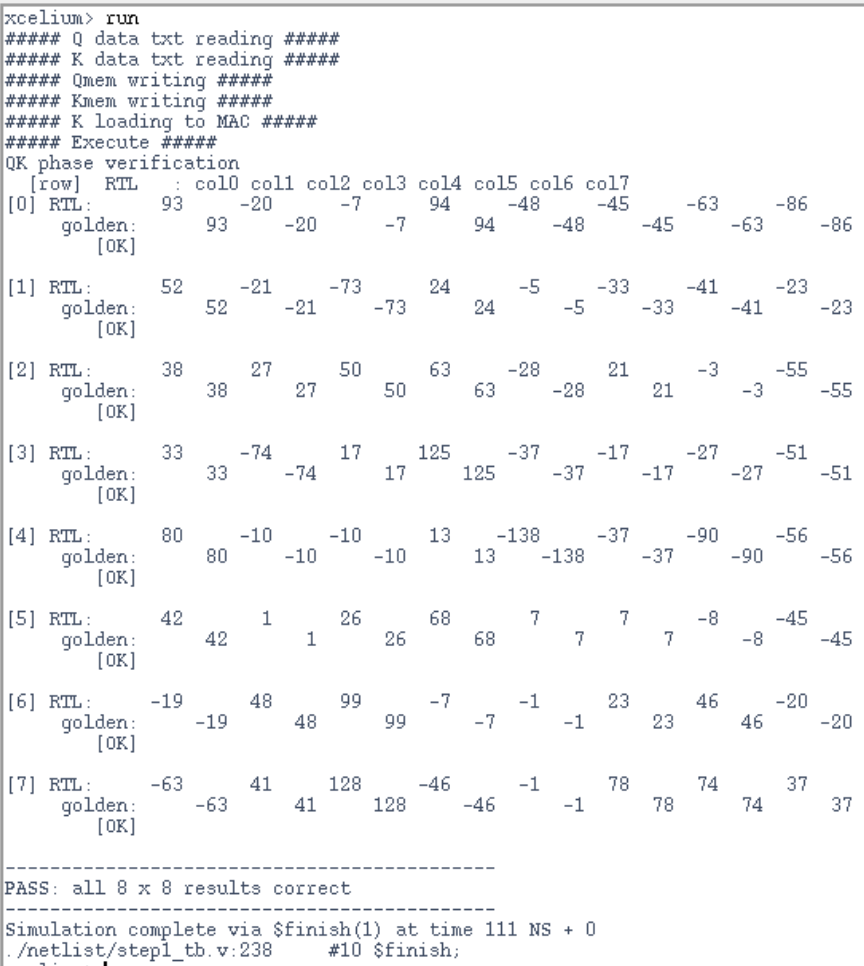
\includegraphics[width=0.30\textwidth]{Step1_images/Step1TO.png}}
    \caption{Single-Core GLS Terminal Output.}
    \label{fig:s1_term}
\end{figure}

\begin{table}[htbp]
    \caption{Step 1 Results}
    \begin{center}
        \begin{tabular}{|c|c|c|c|}
            \hline
            \textbf{} & \textbf{Power (VCD)} & \textbf{WNS} & \textbf{DRC} \\
            \hline
            Single Core & 50.74 mW & -0.014 & 0 \\
            \hline
        \end{tabular}
        \label{tab:s1}
    \end{center}
\end{table}

% ═══════════════════════════════════════════════════════════════════════════
\section{Step 2: Output Normalization}
Behavioral simulation waveform and testbench overview (replace \texttt{temp.png} when the final waveform is finalized).

\begin{figure}[htbp]
    \centerline{
\includegraphics[width=0.30\textwidth]{temp.png}}
    \caption{Behavioral Simulation Waveform / TB.}
    \label{fig:s2_wave}
\end{figure}

% ═══════════════════════════════════════════════════════════════════════════
\section{Step 3: Hierarchical Synthesis of Core}
Memory macros and core integration: SRAM blocks (placeholders) followed by hierarchical core layout and GLS results.

\subsection{Submodule and SRAM Layouts}
\begin{figure}[htbp]
    \centerline{
\includegraphics[width=0.30\textwidth]{temp.png}}
    \caption{SRAM\_64b (Qmem \& Kmem) Layout (placeholder).}
    \label{fig:s3_sram64}
\end{figure}

\begin{figure}[htbp]
    \centerline{
\includegraphics[width=0.30\textwidth]{temp.png}}
    \caption{SRAM\_160b (Psum\_mem) Layout (placeholder).}
    \label{fig:s3_sram160}
\end{figure}

\subsection{Core Layout and GLS}
\begin{figure}[htbp]
    \centerline{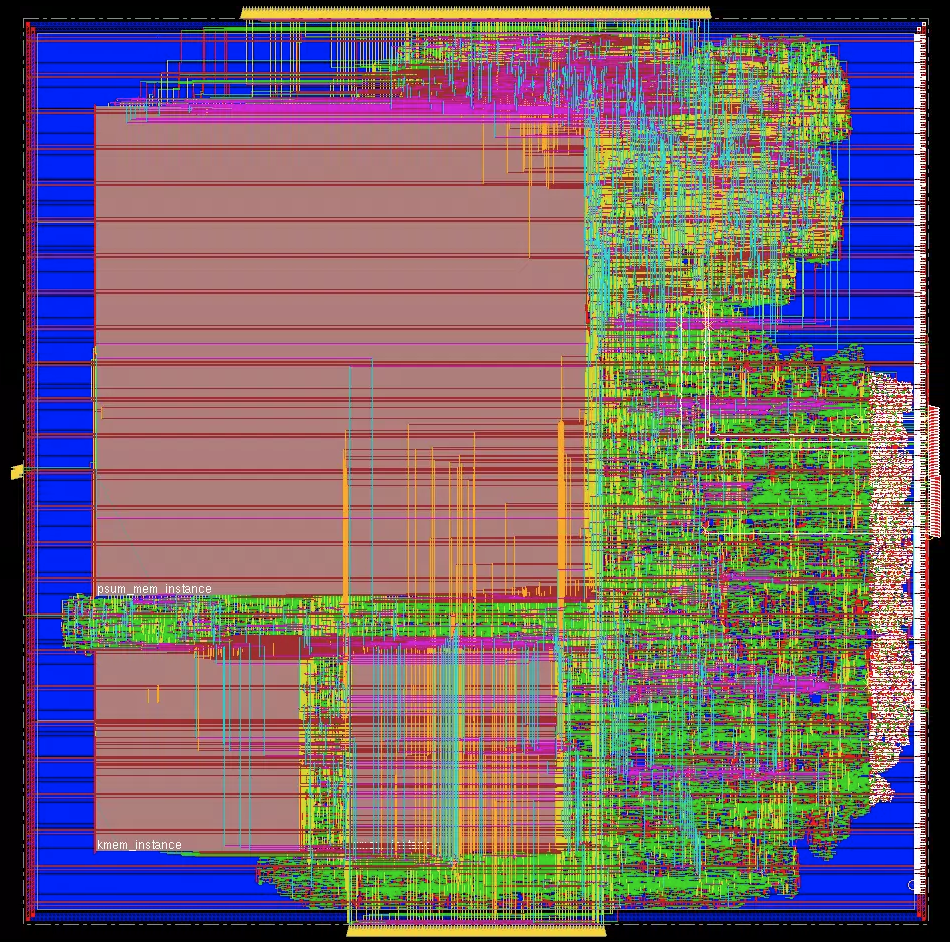
\includegraphics[width=0.30\textwidth]{Step3_images/Step3corelayout.png}}
    \caption{Hierarchical Core Layout.}
    \label{fig:s3_layout}
\end{figure}

\begin{figure*}[htbp]
    \centerline{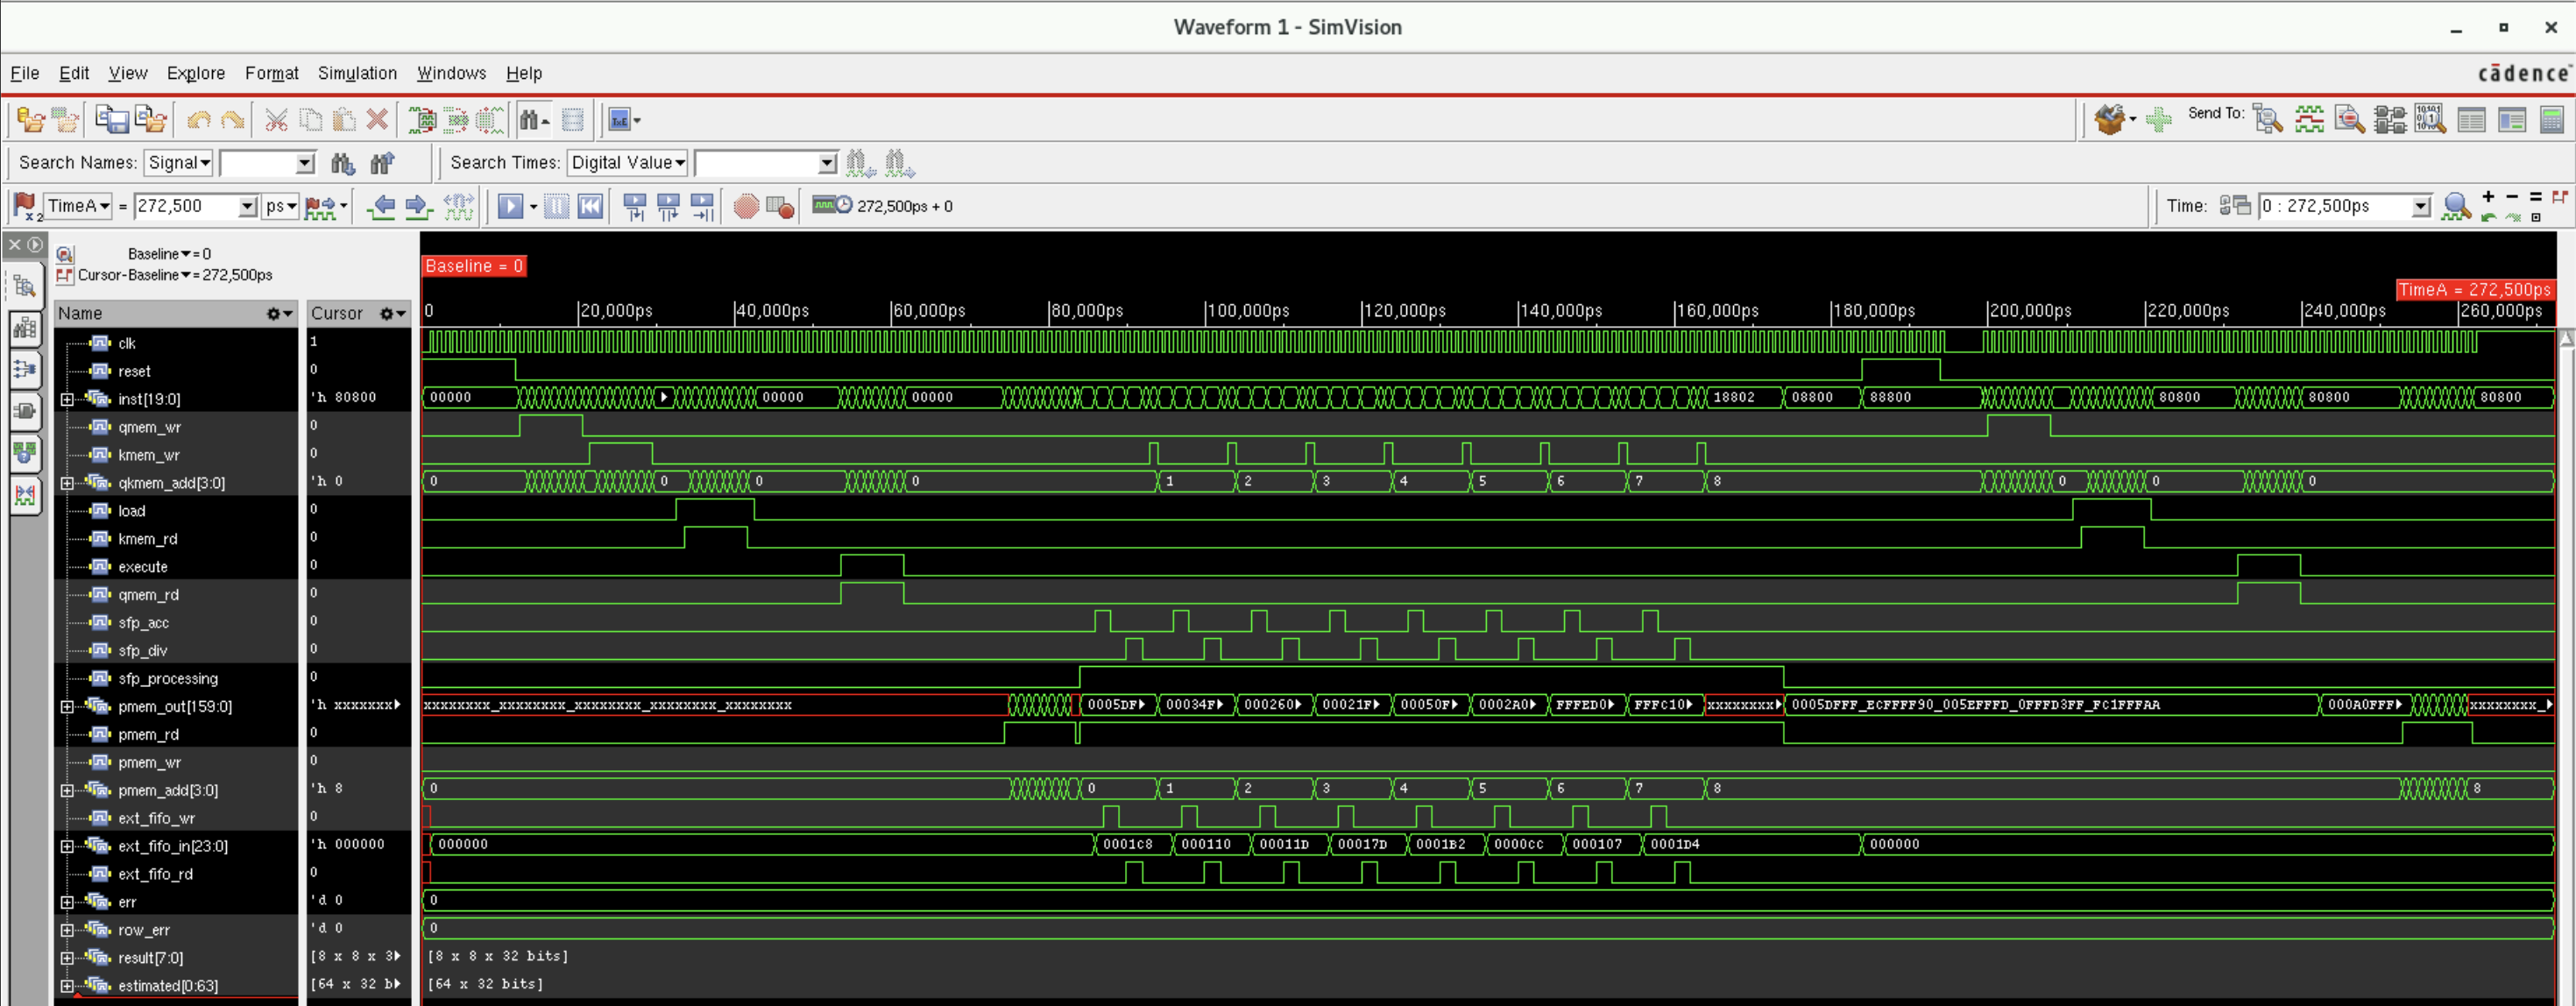
\includegraphics[width=1.0\textwidth]{Step3_images/Step3waveform.png}}
    \caption{Hierarchical Core GLS Waveform.}
    \label{fig:s3_wave}
\end{figure*}

\begin{figure}[htbp]
    \centerline{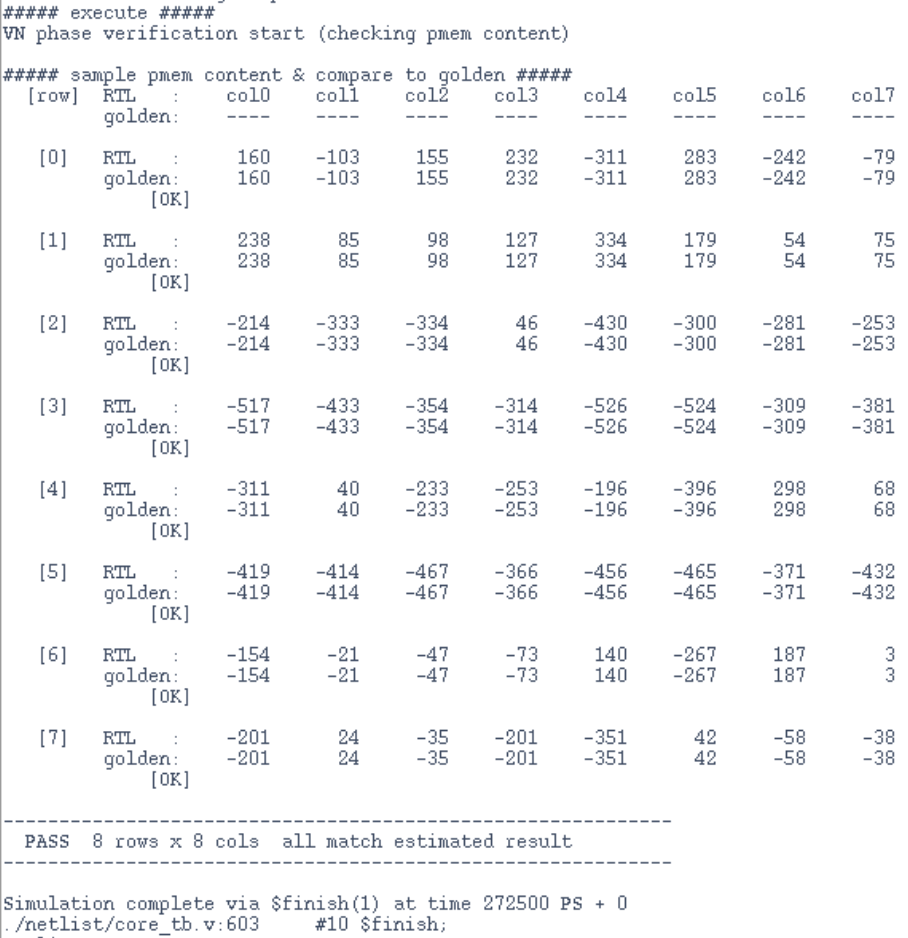
\includegraphics[width=0.30\textwidth]{Step3_images/Step3TO.png}}
    \caption{Hierarchical Core GLS Terminal Output.}
    \label{fig:s3_term}
\end{figure}

\begin{table}[htbp]
    \caption{Step 3 Results}
    \begin{center}
        \begin{tabular}{|c|c|c|c|}
            \hline
            \textbf{} & \textbf{Power (VCD)} & \textbf{WNS} & \textbf{DRC} \\
            \hline
            Hier.\ Core & 61.22 mW & --- & --- \\
            \hline
        \end{tabular}
        \label{tab:s3}
    \end{center}
\end{table}

% ═══════════════════════════════════════════════════════════════════════════
\section{Step 4: Hierarchical Synthesis of Dual-Core}
This milestone includes both fullchip-style views (non-lockstep GLS) and hierarchical dual-core post-PnR results from the LaTeX report.

\subsection{Fullchip / Non-Lockstep GLS (placeholders)}
\begin{figure}[htbp]
    \centerline{
\includegraphics[width=0.30\textwidth]{temp.png}}
    \caption{Fullchip Layout (placeholder; replace with fullchip snapshot).}
    \label{fig:s4_fullchip_layout}
\end{figure}

\begin{figure*}[htbp]
    \centerline{
\includegraphics[width=1.0\textwidth]{temp.png}}
    \caption{Fullchip GLS Waveform, Non-Lockstep (placeholder).}
    \label{fig:s4_nl_wave}
\end{figure*}

\begin{figure}[htbp]
    \centerline{
\includegraphics[width=0.30\textwidth]{temp.png}}
    \caption{Fullchip GLS Terminal Output, Non-Lockstep (placeholder).}
    \label{fig:s4_nl_to}
\end{figure}

\subsection{Dual-Core Post-PnR (lockstep-style assets)}
\begin{figure}[htbp]
    \centerline{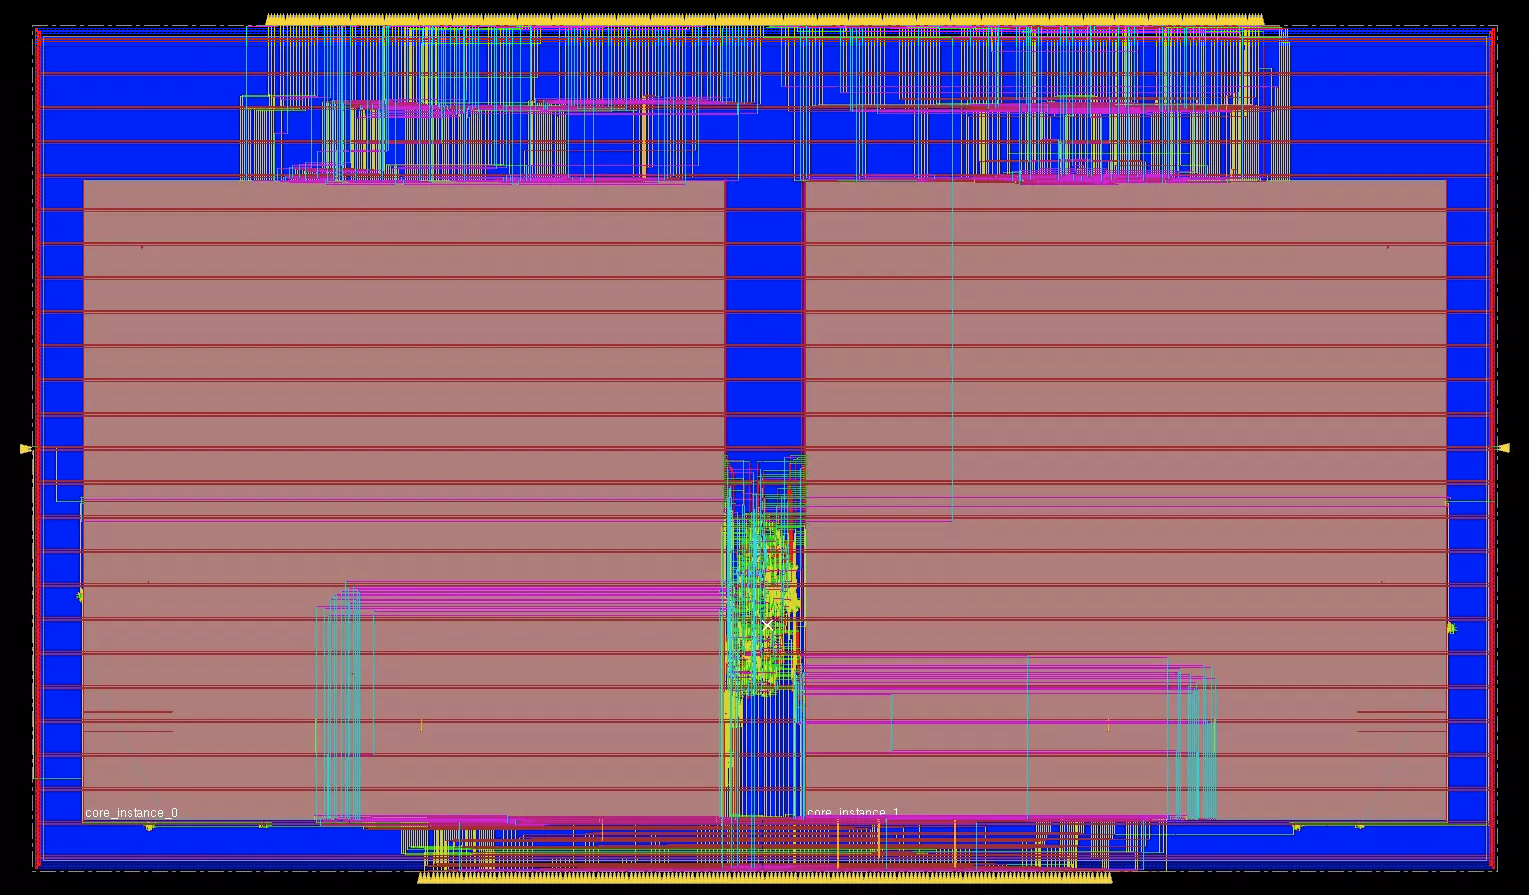
\includegraphics[width=0.30\textwidth]{Step4_images/Step4Layout.png}}
    \caption{Dual-Core Layout.}
    \label{fig:s4_layout}
\end{figure}

\begin{figure*}[htbp]
    \centerline{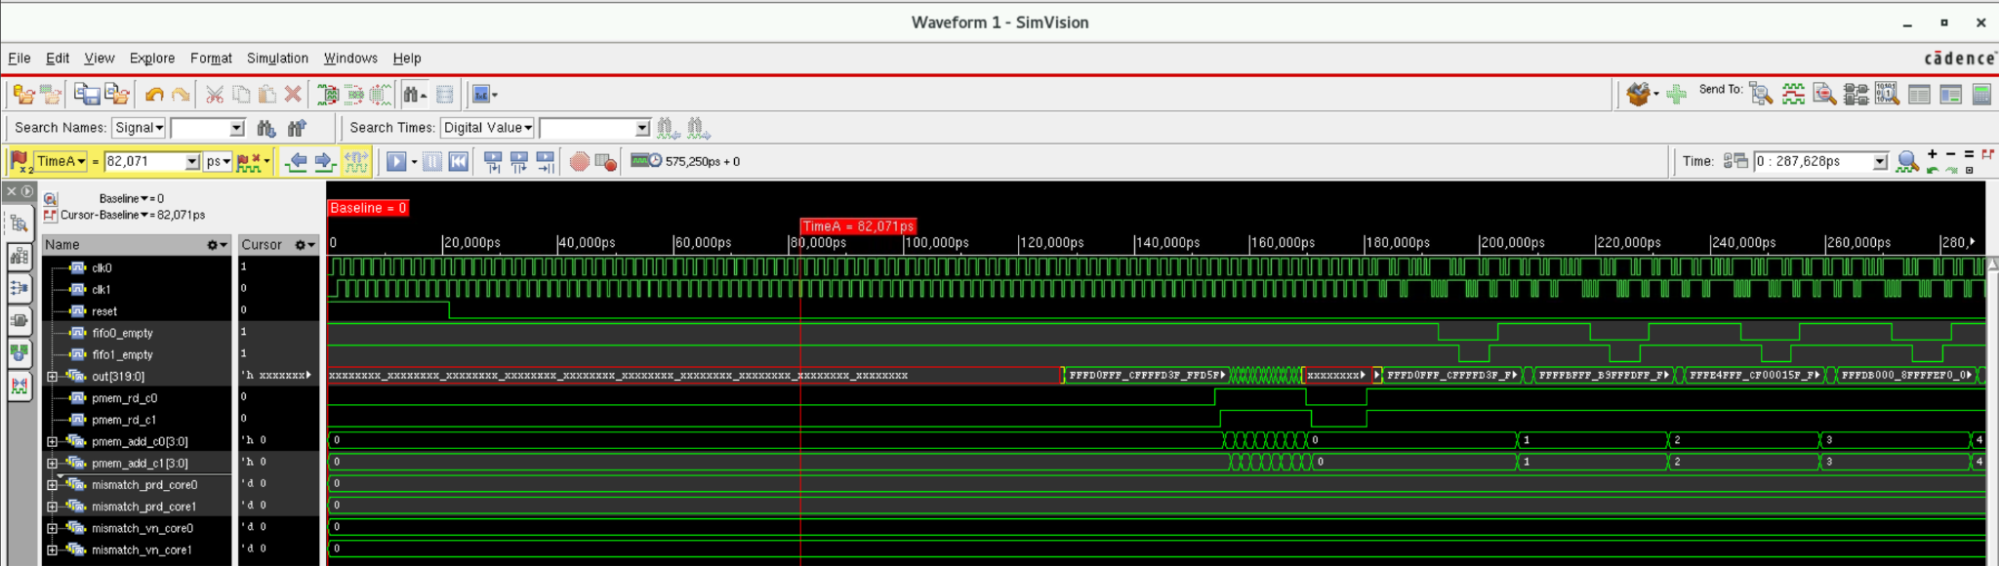
\includegraphics[width=1.0\textwidth]{Step4_images/Step4waveform.png}}
    \caption{Dual-Core GLS Waveform.}
    \label{fig:s4_wave}
\end{figure*}

\begin{figure}[htbp]
    \centerline{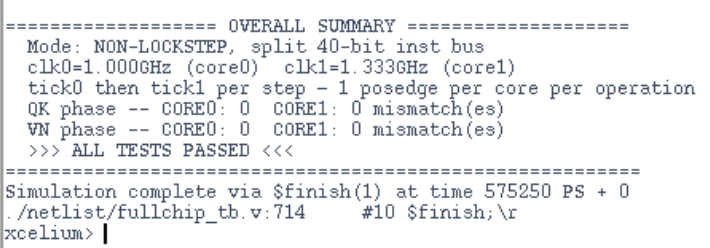
\includegraphics[width=0.30\textwidth]{Step4_images/Step4TO.png}}
    \caption{Dual-Core GLS Terminal Output.}
    \label{fig:s4_term}
\end{figure}

\begin{table}[htbp]
    \caption{Step 4 Results}
    \begin{center}
        \begin{tabular}{|c|c|c|c|}
            \hline
            \textbf{} & \textbf{Power (VCD)} & \textbf{WNS} & \textbf{DRC} \\
            \hline
            Dual Core & 19.19 mW & --- & --- \\
            \hline
        \end{tabular}
        \label{tab:s4}
    \end{center}
\end{table}

% ═══════════════════════════════════════════════════════════════════════════
\section{Step 5: Optimization}
Optimized dual-core figures (placeholders until PnR/GLS images are exported).

\begin{figure}[htbp]
    \centerline{
\includegraphics[width=0.30\textwidth]{temp.png}}
    \caption{Optimized Dual-Core Layout (placeholder).}
    \label{fig:s5_layout}
\end{figure}

\begin{figure*}[htbp]
    \centerline{
\includegraphics[width=1.0\textwidth]{temp.png}}
    \caption{Optimized Dual-Core GLS Waveform (placeholder).}
    \label{fig:s5_wave}
\end{figure*}

\begin{figure}[htbp]
    \centerline{
\includegraphics[width=0.30\textwidth]{temp.png}}
    \caption{Optimized Dual-Core GLS Terminal Output (placeholder).}
    \label{fig:s5_term}
\end{figure}

\begin{table}[htbp]
    \caption{Step 5 Results}
    \begin{center}
        \begin{tabular}{|c|c|c|c|}
            \hline
            \textbf{} & \textbf{Power (VCD)} & \textbf{WNS} & \textbf{DRC} \\
            \hline
            Optimized & --- & --- & --- \\
            \hline
        \end{tabular}
        \label{tab:s5}
    \end{center}
\end{table}

% ═══════════════════════════════════════════════════════════════════════════
\section{Step 6: Hierarchical Sparsity-Aware Attention}
Sparsity-aware dual-core figures (Word title: Sparsity-Aware Attention; placeholders until final images are added).

\begin{figure}[htbp]
    \centerline{
\includegraphics[width=0.30\textwidth]{temp.png}}
    \caption{Sparsity-Aware Attention Dual-Core Layout (placeholder).}
    \label{fig:s6_layout}
\end{figure}

\begin{figure*}[htbp]
    \centerline{
\includegraphics[width=1.0\textwidth]{temp.png}}
    \caption{Sparsity-Aware Attention Dual-Core GLS Waveform (placeholder).}
    \label{fig:s6_wave}
\end{figure*}

\begin{figure}[htbp]
    \centerline{
\includegraphics[width=0.30\textwidth]{temp.png}}
    \caption{Sparsity-Aware Attention Dual-Core GLS Terminal Output (placeholder).}
    \label{fig:s6_term}
\end{figure}

\begin{table}[htbp]
    \caption{Step 6 Results}
    \begin{center}
        \begin{tabular}{|c|c|c|c|}
            \hline
            \textbf{} & \textbf{Power (VCD)} & \textbf{WNS} & \textbf{DRC} \\
            \hline
            Sparsity-aware & --- & --- & --- \\
            \hline
        \end{tabular}
        \label{tab:s6}
    \end{center}
\end{table}

% ═══════════════════════════════════════════════════════════════════════════
\section{Conclusion}
% Add closing discussion after figures and metrics are finalized.

% Include bibliography entries from references.bib without mandatory in-text cites.
\nocite{project_repo}

\bibliographystyle{IEEEtran}
\bibliography{references}

\appendix
\section*{Design Notes (from project outline)}
\addcontentsline{toc}{section}{Design Notes (from project outline)}
\textit{Divider architecture:} pipelined long division vs.\ MCP ``/'' operator; synthesis favored long division; both RTL paths may remain with macro selection (\texttt{SFP\_LONGDIV}, etc.).

\textit{Development flow:} Makefile-driven build, version control (e.g., git), and documented directory layout.

\textit{Interface / controller:} per-core control; example flow---matrix multiply, normalize, read out---with streamlined chip interface hiding unnecessary details from upper-level users.

\end{document}
